\documentclass{article}
\usepackage{amsmath}
\usepackage{amsopn}
\usepackage{graphicx}
\usepackage{amssymb}
\usepackage{geometry}
\geometry{verbose,a4paper,tmargin=25mm,bmargin=20mm,lmargin=15mm,rmargin=20mm}

\DeclareMathOperator{\rect}{rect}
\begin{document}
\author{Martin Kielhorn}
\title{\"Ubung 2 Licht-Mikroskopie (Prof. Heintzmann)}
\maketitle

\noindent Bitte geben Sie diese \"Ubungsserie am 10.\ November 2014 in der Vorlesung ab.

\noindent Nutzen Sie die folgende Definition der Fouriertransformation:
\begin{align*}
  \mathcal{F}\{g(x)\}(k) = G(k) &= \frac{1}{\sqrt{2\pi}}\int_{-\infty}^\infty\!\!\! g(x) e^{-ikx} \textrm{d}x
\end{align*}
F\"ur mehr Dimensionsionen gelte die Definition entsprechend der Vorlesung.

\section{Fouriertransformierte von zwei Funktionen}
Berechnen Sie die Fouriertransformierten der folgenden Funktionen.
\begin{align}
  \rect(x) &=\begin{cases}
  1, & |x|\le 1/2 \\
  0, & |x| > 1/2
  \end{cases}
\end{align}

\begin{align}
  \Theta(x)&=\begin{cases}
  0, & x<0 \\
  1, & x \ge 0
  \end{cases}
\end{align}
Hinweise:
\begin{itemize}
  \item $\Theta'(x)=\delta(x)$
  \item  Eigenschaften der Fouriertransformation bei Ableitung einer Funktion
  \item $\int_0^\infty \frac{\sin k}{k}\textrm{d}k=\pi/2$. Dieses
    Integral ist n\"utzlich bei der Bestimmung von
    $\mathcal{F}^{-1}\{1/k\}$.
\end{itemize}

\section{Faltungstheorem}
Es seien $\mathcal{F}\{f(x)\}(k)=F(k)$, $\mathcal{F}\{g(x)\}(k)=G(k)$ und die Faltung $F(k)\otimes G(k)=\int_{-\infty}^\infty\!\!\!\! F(\xi)G(k-\xi)  \textrm{d}\xi$. Zeigen Sie:
\begin{align}
  \mathcal{F}\{f(x)\cdot g(x)\} &= F(k)\otimes G(k)
\end{align}


\section{Laplace Operator}
Zeigen Sie, dass der zweidimensionale Laplace Operator $\nabla^2 =
\partial^2/\partial x^2 + \partial^2/\partial y^2$ im Fourierraum
proportional zu einer Multiplikation mit einem quadratischen Funktion
des Wellenvektors $k$ ist:
\begin{align}
  \mathcal{F}\{\nabla^2 g(x,y)\} &\propto (k_x^2+k_y^2) \mathcal{F}\{g(x,y)\}
\end{align}

\section{Nerdmemory}
Ordnen Sie die Pupillenmasken $(i-xx)$ ihren Fraunhofer-Beugungsmustern $(a-t)$
(Fotographien der 2D Leistungsdichtespektren) zu. Hinweis: Nutzen Sie die
aus der Vorlesung bekannten Eigenschaften der
Fouriertransformation. Die Bilder sind m\"oglicherweise gegeneinander
verdreht.

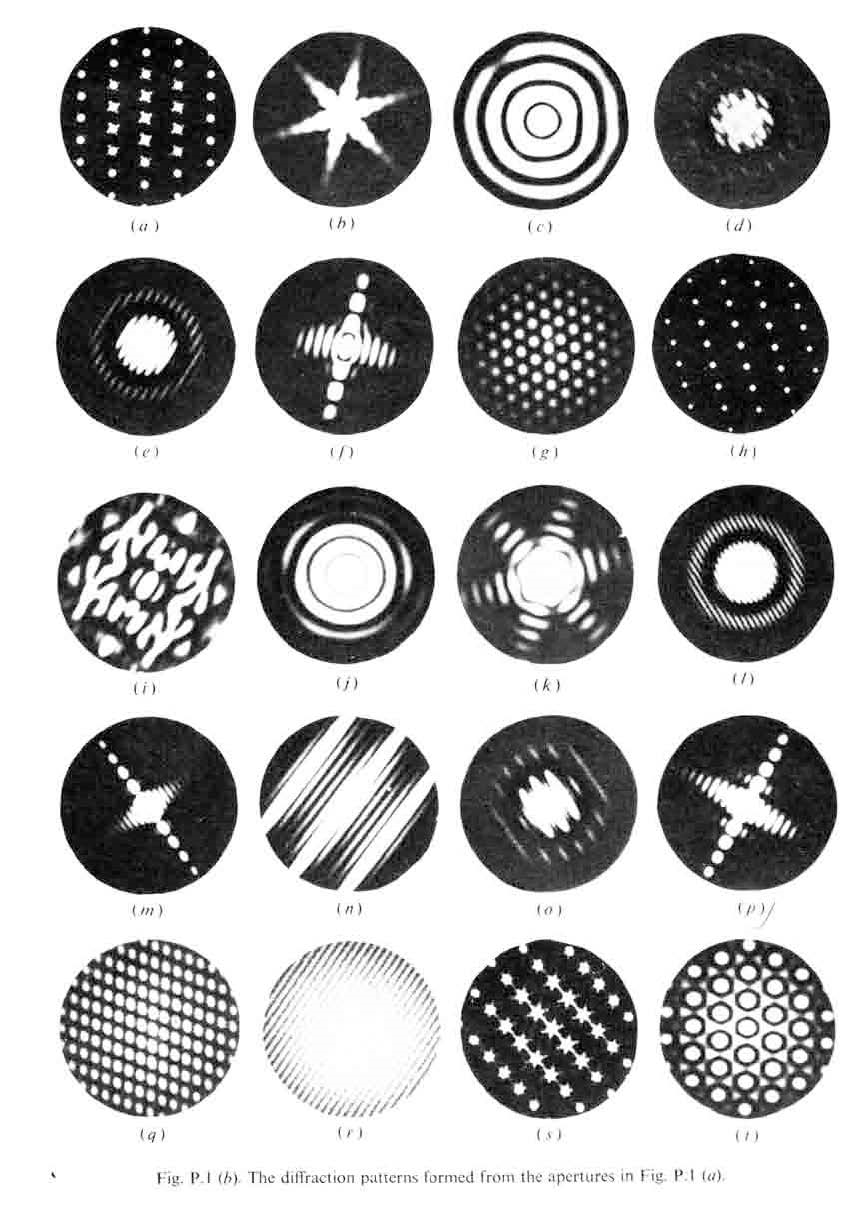
\includegraphics[height=.72\textheight, angle=90]{FrequencySpace}

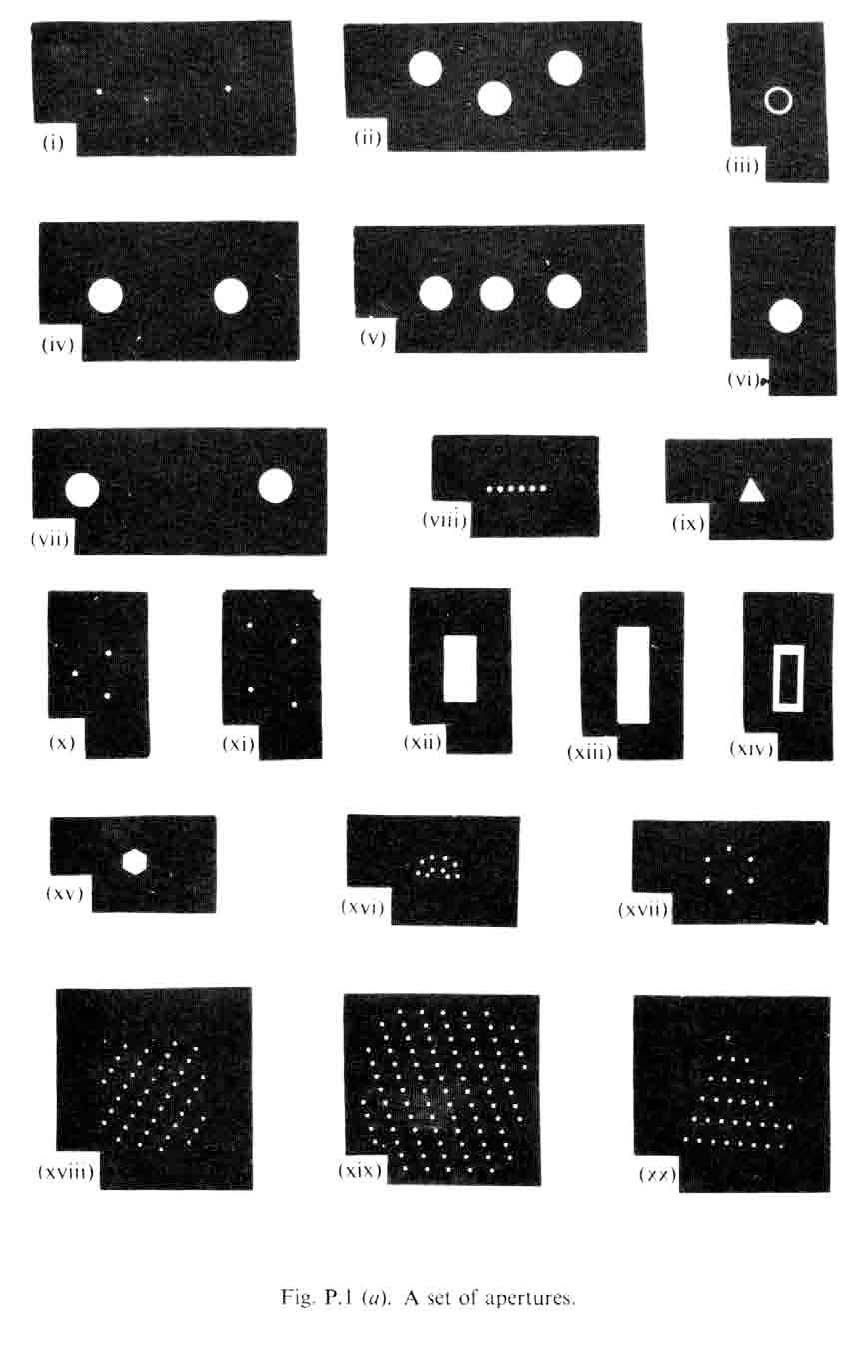
\includegraphics[height=.72\textheight, angle=90]{RealSpace}

{\tiny Die Bilder stammen aus einem Kurs von Brad Amos.}

\end{document}
